\chapter*{Preface}

Since its inception in the early 1980s,
\emph{diffeology} has become an alternative to
---or rather an extension of---
traditional differential geometry.
With its developments in higher homotopy theory,
fiber bundles,
modeling spaces,
Cartan-de Rham calculus,
moment maps and the symplectic program,
for example,
diffeology now covers a large spectrum of traditional fields and deploys them from singular quotients to infinite-dimensional spaces
---and sometimes mixes the two---
treating mathematical objects that are or are not strictly speaking manifolds,
and other constructions,
on an equal footing in a common framework.

We shall see some of its achievements through a series of examples,
chosen because they are not covered by the geometry of manifolds,
because they involve infinite-dimensional spaces or singular quotients,
or both.

The growing interest in diffeology comes from the conjunction of two strong properties of the theory:

(1) First of all,
the category \Category{Diffeology} is stable under all set-theoretic constructions:
sums,
products,
subsets,
and quotients.
One says that it is a complete and co-complete category.
The space of smooth maps in diffeology has itself a natural \emph{functional diffeology} for which the category is also Cartesian closed.
This allows us to treat spaces of smooth maps between spaces as ordinary spaces.
Mathematicians appreciate these kinds of categories for their stability with respect to set-theoretic constructions.

(2) Just as important:
quotient spaces,
even heavily non-Hausdorff,
Sikorski or Frölicher \cite{KM97} etc.,
acquire a natural,
non-trivial,
and meaningful diffeology.
This is particularly true of the \emph{irrational tori},
where it all began:
non-Hausdorff quotients of the real line by a dense subgroup.%
\footnote{More generally,
quotients of Euclidean spaces $\RR^n$ by generating dense and discrete (in the sense of diffeology) subgroups.
They are also quotients of ordinary tori $\Torus^n$ by dense foliations.}
They possess,
as we shall see,
a non-trivial diffeology,
capturing faithfully the intricacy of the subgroup within its ambient space.
This crucial property will be the raison d'être of many new constructions,
or wide generalizations of classical constructions,
that cannot exist in almost all other extensions of differential geometry.%
\footnote{The kind of spaces that are trivial under the various generalizations of $\Cinfty$ differential geometry:
I am not considering the various algebraic generalizations that do not play on the same level of intuition and generality and do not concern exactly the same sets/objects.
We are indeed interested in differential geometry in the broadest sense.}

The handling of any kind of singularities,
maybe more than the inclusion of infinite-dimensional spaces,
reveals how diffeology changes the way we understand smoothness and discriminates this theory among the various alternatives.
See,
for example,
the use of dimension in diffeology,%
\footnote{See \cite{PIZ07}.}
which distinguishes between the different half-lines,
quotients $\RR^n\!/\O(n)$,
on a pure differential geometry level.

In this regard,
we can distinguish several types of singularities:

(a) A space can be singular when it presents a fatal mismatch between its topology and its diffeology,
as in the case of the irrational torus.

(b) A point in a space can be singular when it behaves differently from other points under the action of diffeomorphisms.
This is what happens in orbifolds,
for example.

(c) A point in an embedding can behave differently from other points under the action of ambient diffeomorphisms.
This is the case of the cusp in the semi-cubic.

Figure \ref{The-Scope-of-Diffeology} shows the inclusivity of diffeology,
with respect to differential constructions,
in comparison with the classical theory.

\begin{figure}[t]
  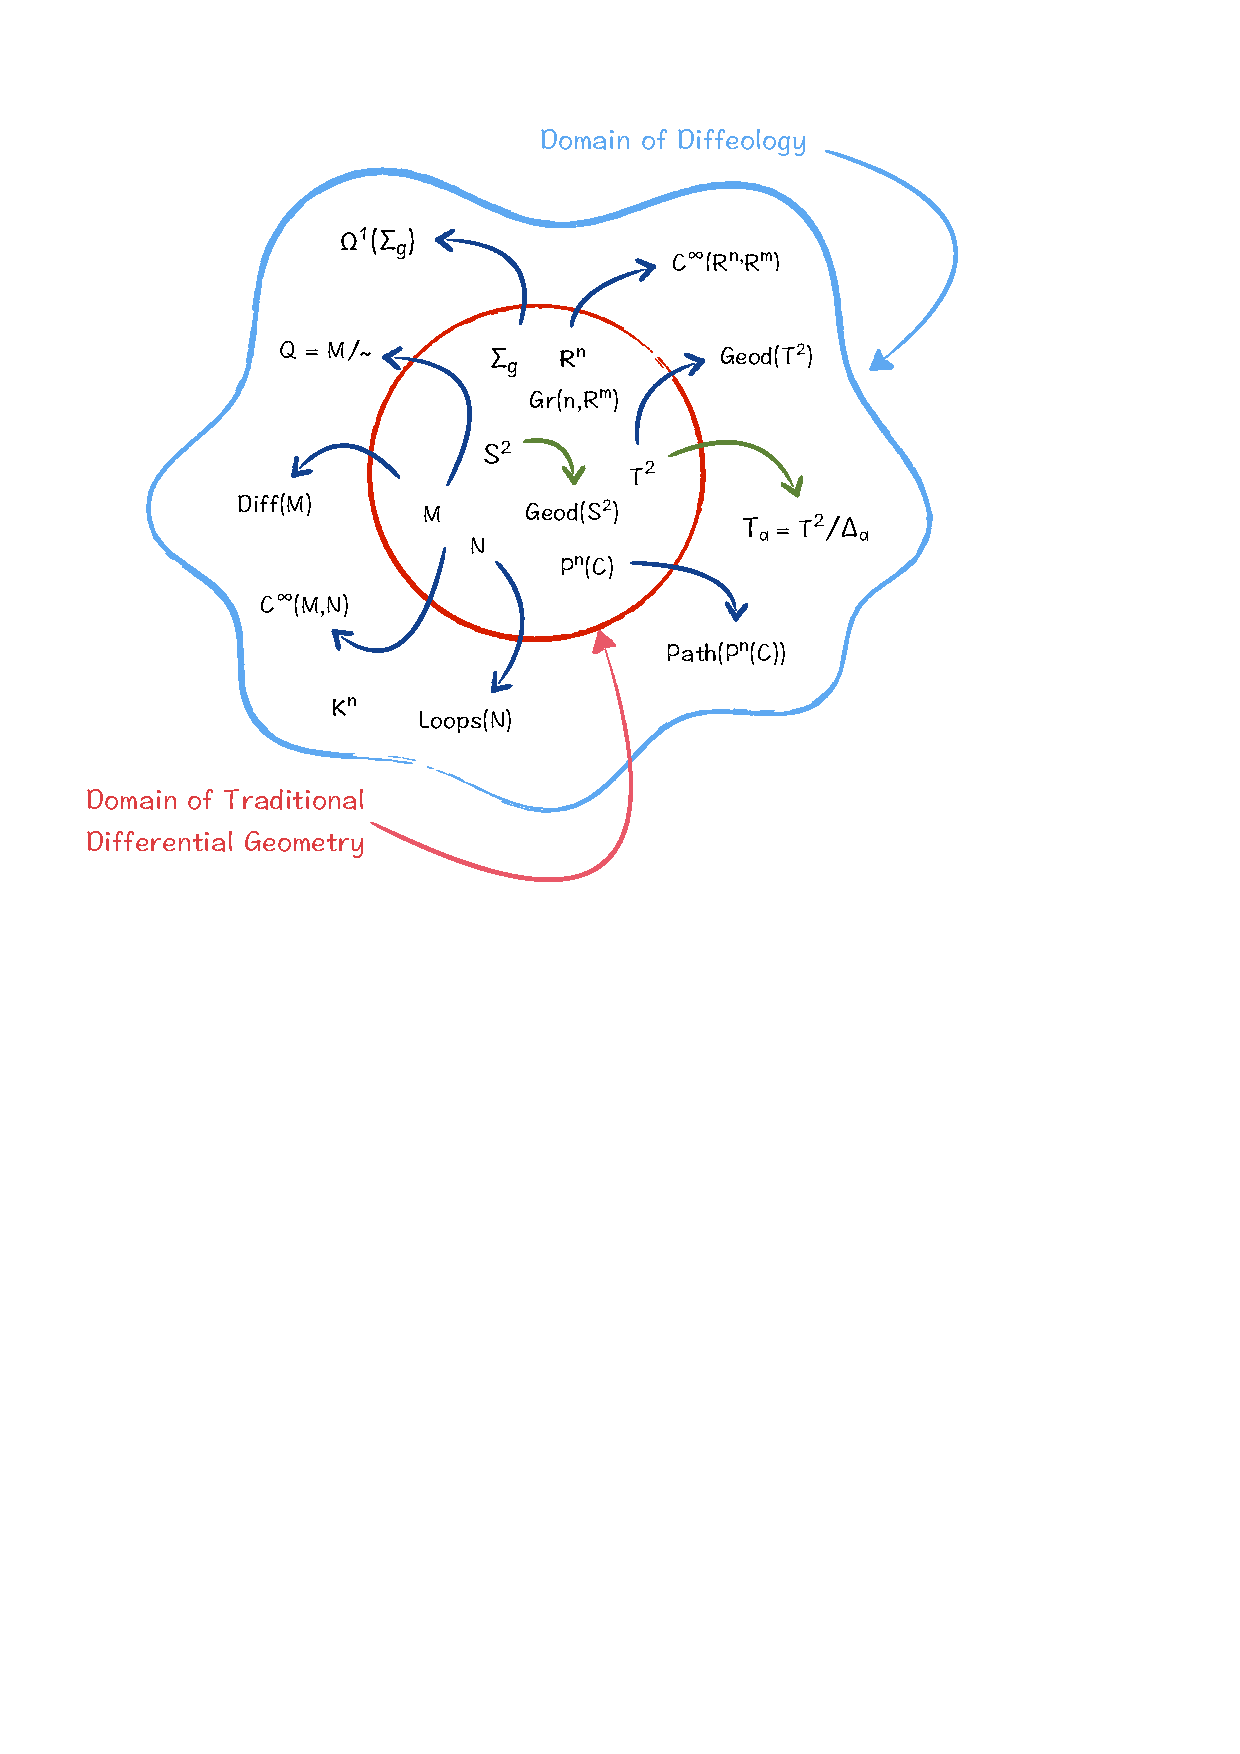
\includegraphics[width=.75\textwidth]{Figures/The-Scope-of-Diffeology.pdf}
  \vspace{-.25\baselineskip}
  \caption{The scope of diffeology.}
  \label{The-Scope-of-Diffeology}
\end{figure}

The story began in the early 1980s,
when Jean-Marie Souriau introduced his axiomatics called \emph{difféologies} in a paper titled ``Groupes Différentiels'' \cite{Sou80}.
It was defined as a formal yet lightweight structure on groups,%
\footnote{Compared to heavy structures in functional analysis.}
and it was designed for dealing easily with infinite-dimensional groups of diffeomorphisms,
in particular the group of symplectomorphisms or quantomorphisms.
He named the groups equipped with such a structure \emph{groupes différentiels},%
\footnote{Which translates into English as ``differential'' or ``differentiable groups.''}
as announced in the title of his paper.%
\footnote{Actually,
difféologies are built on the model of K.-T. Chen's \emph{differentiable spaces} \cite{Che77},
for which the structure is defined over convex Euclidean subsets instead of open Euclidean domains.
That makes diffeology more suitable to extending differential geometry than Chen's differentiable spaces,
which focus more on homology and cohomology theories.}
His definition was made of five axioms that we can decompose today into the first three that later gave the notion of diffeology on arbitrary sets,
and the last two,
for the compatibility with the internal group multiplication.
But it took three years,
from 1980 to 1983,
to separate the first three general axioms from the last two specific ones and to extract the general structure of \emph{espace différentiel} from the definition of \emph{groupe différentiel}.
It is in particular the results on the \emph{irrational torus} \cite{DI83} and the development of homotopy \cite{Igl85}
that made urgent and unavoidable a formal separation between groups and spaces in the domain of Souriau's \emph{differential structures},
as that gave a new spin to the theory as we know it today.%
\footnote{I talk more on this story in the postface.}

Since its inception,
the theory has evolved significantly and the book {\it Diffeology} is certainly a reference for the basic areas of the theory.
I refer to it as the ``textbook'' in the following \cite{PIZ13}.

This book,
{\it Lectures in Diffeology},
does not play the same role;
it is not a rewrite of the textbook despite having the same basis.
The first half consists of notes from a series of lectures I gave at Shantou University in 2020/21,
at the initiative of Enxin Wu,
as part of a Chinese program for visiting professors.
Writing down the lecture notes was part of the contract.
In writing them,
I have tried not to copy verbatim (although this is sometimes unavoidable) parts of the textbook,
as it is more a support for these lectures.
Instead,
I have tried to extract the spirit of the constructions rather than their formalization.
Readers can always refer to the relevant passage in the textbook for further details.
I have tried to highlight the most important constructions that underpin the various branches of differential geometry,
such as homotopy,
fiber bundles,
differential calculus,
and so on.
And to show how they morph into diffeology,
what makes them similar and what makes them different from what we are used to.

The second part of the book is a series of blog notes I have posted on my website.
These are various notes,
remarks,
or exercises that I felt were interesting enough to share.
I hope they will encourage some readers to develop the ideas or constructions they introduce.
I am thinking in particular of Riemannian diffeology,
which is still only a program.
Symplectic diffeology,
which is already well-developed,
still needs more thought before it can become a mature theory.
I have not been able to incorporate the recent developments and example of \v{C}ech cohomology that I have presented elsewhere;
perhaps a future edition of these lectures will do justice to this issue.

And,
because this book is more a work in progress than a finished thought,
I decided to present it as a series of typed notes,
which explains its particular layout and the choice of typography.

\smuline{On an entirely different note},
the special properties of diffeology:
complete,
co-complete,
and Cartesian closed,
have made this category a tool of choice for categoricians,
especially in \emph{differential homotopy} and \emph{model categories}.%
\footnote{I cite just a couple of names in these subfields in rapid development,
for example \cite{CW14} in model categories,
and \cite{SYH18, Kih19, Kur20} in differential homotopy.}
Japan and China have taken the lead in these two fields,
which deserves to be mentioned.
I asked Enxin Wu to contribute to this book on the subject.
He graciously accepted to write a short text which I have appended as a first step in this direction.

\smuline{In conclusion},
I will try to say why,
from my point of view,
diffeology is the perfect framework for differential geometry,
to the point that it is exactly what we expect differential geometry to be.
First of all,
the geometer will find pleasant and useful the flexibility of diffeology
to extend,
in a unique formal and versatile framework,
different constructions in various fields,
without inventing a heuristic framework each time that momentarily satisfies their needs.

Then,
beyond all these circumstances and technicalities,
what does diffeology have to offer on a more formal or conceptual level?
The answer lies partly in Felix Klein's Erlangen program \cite{Kle72}:

\begin{quote}
  The totality of all these transformations we designate as the {\it principal group} of space-transformations;
  {\it geometric properties are not changed by the transformations of the principal group}.
  And,
  conversely,
  {\it geometric properties are characterized by their remaining invariant under the transformations of the principal group}\dots
  
  As a generalization of geometry arises then the following comprehensive problem:
  
  {\it Given a manifoldness and a group of transformations of the same;
  to investigate the configurations belonging to the manifoldness with regard to such properties as are not altered by the transformations of the group.}
\end{quote}

As we know,
these considerations are today regarded by mathematicians as the modern interpretation of the word/idea of \emph{geometry}.
A geometry is given as soon as a space and a group of transformations of this space are given.%
\footnote{Jean-Marie Souriau reduces the concept of geometry to the group itself \cite{Sou03}.
But this is an extreme point of view I am not inclined to share,
for several reasons.}

Consider,
for example,
Euclidean geometry,
defined by the group of Euclidean transformations,
our {\em principal group},
on the Euclidean space.
We can interpret,
for example,
the {\em Euclidean distance} as the invariant associated with the action of the Euclidean group on the set of pairs of points.
We can superpose a pair of points onto another pair of points,
by an Euclidean transformation,
if and only if the distance between the points is the same for the two pairs.%
\footnote{We could continue with the case of triangles and other elementary constructions
--~circles,
parallels etc.~--
involving the nature of stabilizers.
We can compare between Euclidean and symplectic geometry,
for example,
from a strict Kleinian point of view.
See the discussion in \cite{PIZ02}.}
Hence,
{\em geometric properties} or {\em geometric invariants} can be regarded as the orbits of the {\em principal group} in some spaces built on top of the principal space,
and also as fixed/invariant points,
since an orbit is a fixed point in the set of all the subsets of that space.
In brief,
what emerges from these considerations suggested by Felix Klein's principle is the following:

\smuline{Claim.}~A geometry is associated with/defined by a {\em principal group} of transformations of some space,
according to Klein's statement.
The various geometric properties/invariants are described by the various actions of the principal group on spaces built on top of the principal space:
products,
sets of subsets,
and so on.
Each one of these properties,
embodied as orbits,
stabilizers,
quotients,
and so on,
captures a part of this geometry.

Now,
how does diffeology fit into this context?

$*$ One can regard a diffeological space as the collection of the plots that gives its structure.
This is the {\em passive approach}.

$*$ Or we can look at the space through the action of its group of diffeomorphisms%
\footnote{We consider more precisely the action of the pseudo-group of local diffeomorphisms.}
on itself,
but also on its powers or parts or maps.
This is the {\em active approach}.

This dichotomy appears already for manifolds,
where the change of coordinates (transition functions of an atlas) is the passive approach.
The active approach,
as the action of the group of diffeomorphisms,
is often neglected,
and there are a few reasons for that.
Among them,
the group of diffeomorphisms is not a Lie group {\em stricto sensu}
--~it does not fit in the category \Category{Manifolds}~--
and that creates a psychological issue.
A second reason is that its action on the manifold itself is transitive,%
\footnote{Generally,
manifolds are regarded as connected,
Hausdorff,
and second countable.}
there are no immediate invariants,
one having first to consider some secondary/subordinate spaces to make the first invariants appear.

These obstacles,
psychological or real,
vanish in diffeology.
First of all,
the group of diffeomorphisms is naturally a diffeological group.
And the square,
discussed in one of the lectures,
is an example of a space where the action of the group of diffeomorphisms,
the main group in Klein's sense,
captures a good first image of its geometry.%
\footnote{And not just of its topology.}
Indeed,
it has three orbits:
the corners,
the edges,
and the interior.
Any diffeomorphism preserves separately the interior of the square and its border,
which is a consequence of the D-topology.%
\footnote{A diffeomorphism is in particular a homeomorphism for the D-topology.
This is an opportune moment to emphasise this:
the diffeology approach is that topology is a consequence of differential structure,
and not the other way round as it is usually the case,
where the differential structure is subordinate to the topology.}
But the fact that a diffeomorphism of the square cannot map a corner into an edge is a typical smooth property.

Klein's principle can already be tested on this simple example.
As the square is naturally an object of the theory,
there is no need for a heuristic extension here.

\smuline{Claim.} Considering the group of diffeomorphisms of a diffeological space as its principal group,
we can look at diffeology as the formal framework that makes {\em differential geometry},
\smuline{the geometry} ---~in the sense of Felix Klein~--- \smuline{of the group of diffeomorphisms}.
Or possibly,
the (larger) pseudogroup of local diffeomorphisms.%
\footnote{In comparison with \cite{Sou03}.}

Actually,
the action of local diffeomorphisms defines a stratification,
called \emph{Klein stratification},
that embodies the internal geometry of the object itself.
The general geometry to which it belongs is defined by the specific category of objects to which it is formally attached.
For example,
Euclidean geometry becomes the category of Euclidean objects,
that is,
the category of spaces equipped with an action of the Euclidean group with morphism equivariant maps.

Because diffeology is such a wide and stable category that satisfactorily encompasses so many diverse situations,
from singular quotients to infinite dimensions,
even mixing cases,%
\footnote{See \cite{PIZ16},
for example.}
I think it is fair to say that it largely fulfils its mission and,
according to the Kleinian viewpoint,
answers the question once posed by a student:
"In what way is diffeology geometry?"

\smuline{\bf A refinement of Souriau's radical stance.}
Souriau famously claimed that ``le groupe est la géométrie'' \cite{Sou03},
extending Klein's Erlangen Program to encompass all of differential geometry.
To achieve this,
he had to enlarge the category of manifolds to include infinite-dimensional diffeomorphism groups,
and diffeology was the tool he created for this purpose.
However,
a recent work
---~the Boman Paradox~---
has forced me to refine this view.
As we shall see in Chapter B25,
there exist two diffeological spaces with identical topology and identical abstract diffeomorphism groups
that are nevertheless geometrically distinct.
The missing ingredient is the local smooth structure,
which precedes the group and cannot be recovered from it.
Thus, while the Kleinian--Souriau perspective is a powerful guide,
it is not the final word.
Diffeology reveals that the space determines the group,
but the group
---~even as a diffeological group~---
does not determine the space.
The arrow of definition is irreversible.
